\documentclass[11pt]{article}
\usepackage{fullpage}
\usepackage{graphicx}
\usepackage{natbib}
\usepackage{hyperref}

\begin{document}
\title{Radio Skillz: Digital Lab 1}

\maketitle

\section*{Prerequisites}

\begin{itemize}
\item Nyquist Sampling
\item Data Representations
\item Quantization and Rounding
\end{itemize}

\section*{Materials}

\begin{itemize}
\item ROACH board
\item quad-ADC board
\item 200 MHz clock source
\item 0-400 MHz tone generator
\item noise generator
\item various low-pass and band-pass filters
\end{itemize}

\section*{Some Thoughts}

\subsection*{FPGAs and Simulink}

We're just getting started on our digital part of the class, and we haven't really had a chance to talk
about Field Programmable Gate Arrays (FPGAs) or how they are programmed --- that's going to come next
week.  However, we're going to use one today, so let's cover what you need to know.

\subsubsection*{The ROACH}

The Reconfigurable Open Architecture for Computing Hardware (ROACH) is an open-source board (e.g.
all schematics, board design, etc. are free and open) developed by the CASPER collaboration, which
is now pan-global.  On this board is a Virtex-5 FPGA made by Xilinx, along with a CPU.  The CPU
runs linux (you can ssh into it), using a special linux kernel cooked up by CASPER that allows it to support 
automatic interfaces to some of the logic you program the FPGA with.

FPGAs are programmed with ``bit files'' that you load onto the chip, and tell the circuitry inside what
wires to connect to what logic components.  To load a bit file onto the ROACH FPGA, you execute a *.bof file
from the CPU.  The BOF file contains both a bit file, as well as some other information that allows
linux to interface to the FPGA.  After running a BOF file (leave it running), you need to find the 
process ID of that program.  The linux command ``jobs'' should do the trick.

\begin{figure}\centering
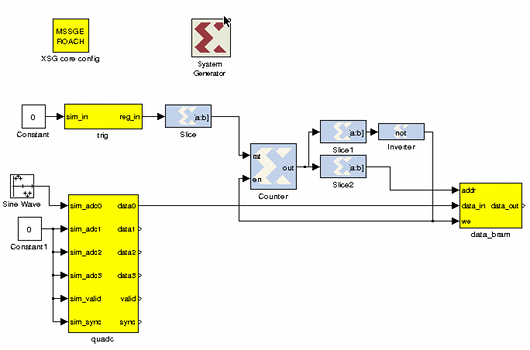
\includegraphics[width=6in]{digital_lab_1_plots/adc_capture.png}
\end{figure}

Finally, if you go to a secret directory /proc/PID/hw/ioreg (where PID is the process ID), you'll find
a bunch of files that have names that correspond to some of the blocks in the schematic diagram above.
The schematic above is an actual FPGA program.  It tells the FPGA to read samples from an interface to
the quad-ADC (described below), and place them into a BRAM (block random access memory) until it is full.
The address to which samples are written is supplied by a counter that stops itself at the final address
of the BRAM, and waits for a signal to come in over the register ``trig'' to reset the counter back to
0 and allow it to write new samples in into the memory.  You'll notice that ``trig'' and ``data\_bram''
are files in the ioreg directory; those are your interfaces to the register that triggers a data capture,
and the data itself that is written into the BRAM.  You can write a value to the file ``trig'', and you can
read values out of the file ``data\_bram'', just as if they actually were files.  But they are not.  They
are interfaces to the FPGA.  But Python doesn't know that.

So all you need to know now is this: that ``trig'' is an unsigned 32-bit integer, and the least-significant bit
controls the counter reset button.  The BRAM holds signed 32-bit samples for each ADC sample.  The
ADC is natively an 8-bit sampler, and its sample clock is controlled by a function generator feeding the
SMA port marked ``clk''.  Happy sampling.

\subsection*{Writing Code for Lab}

As last week, please put the code you develop for this lab
in your class Git repository.  You'll add to named directory the files ``van\_vleck.py''.

\section{Sampling and Aliasing}

\subsection{Starting Your ROACH}

Transfer the *.bof file in the class repository over to the ROACH as before,
and run it.  Make sure the sample clock to the ADC is set to 200 MHz, and is
on before you program the FPGA.  FPGAs behave very erratically if they aren't
clocked properly; if you program the FPGA and then turn on the clock, you may
see gibberish, or even nearly-correct behavior that occasionally goes whacky.
Also check that you have attached anoise signal into the ADC, so that you get
something interesting in your BRAM.  

\subsection{Running the Design}

You can now write appropriate values to "trig" to initiate a data capture.  You
can use ``hd'' to look at values in "data\_bram" and make sure things make sense.
When you are happy with the contents of the BRAM, you can scp the file over to
another computer, freeing up the ROACH for someone else.

\subsection{Sampling a Tone}
\begin{itemize}
\item use the quad-ADC attached to the ROACH to sample input tones at 200 MHz.
\item capture data for three tone
frequencies: one that has dozens of samples per period, one that is 10\% below the Nyquist frequency,
and one that is 10\% above the Nyquist frequency.
\item predict the frequencies you expect for these tones after you sample them.
\item write a python program (plot\_adc\_samples.py) that plots the data as it sits in binary format
in the file.  You might want to take a look at the ``struct'' module.  Try your best to set the time
axis with proper units.
\item measure the frequencies of the various tones, and compare them to your predictions.
\end{itemize}

\subsection{Sampling Band-limited Noise}
\begin{itemize}
\item use low-pass and band-pass filters to inject noise (your amplifier chains from the previous
lab are great noise sources) into the first and second nyquist zones of your digitizer.  Since there
may be only a limited selection of filters available, it may be easier change your sampling
frequency to match your filter.
\item capture the data and plot the (aliased) spectrum for each case.  Again, try your best to get your
frequency units right.  Put your plotting script in your repo under plot\_adc\_
\item transpose the measured spectrum up to the original frequency.  Compare features to what you expect
given your choice of filters.
\end{itemize}

\section{Compu-Acting}

In this class activity, we'll act like various processors.  Fun.

\section{Quantization Power Transfer}

\begin{itemize}
\item write code in van\_vleck.py that plots the power transfer curves for 1, 2, 4, and 8-bit sampling.
\end{itemize}

\end{document}
